% !TEX root = ../main.tex
\chapter{Event Contracts and a Regulated Exchange}\label{ch:kalshi}
\begin{paracol}{2}

\begin{sources}
\begin{tabularx}{\linewidth}{@{}l l L@{}}
\toprule
\textbf{Lecture} & \textbf{Speaker} & \textbf{Content}\\
\midrule
2024 L20 & T.~Mansour (Kalshi), guest; introduced by P.~Kempthorne & Why an exchange for events; the three-year regulatory road and the lawsuit against the regulator; betting market versus exchange; arbitrage against other assets; cash collateral and margin; who trades (institutions, retail); revenue model; market makers and quoted spreads; career advice. Questions from students and from J.~Xia and V.~Strela.\\
\bottomrule
\end{tabularx}

\smallskip
\textbf{Files.} None: only the video transcript exists for this lecture (no slides, no notes, no
problem set). Everything attributed to the lecture below is taken from the spoken words, and the
tags \ts{24}{20}{0:00}~point into the video. The company facts (volumes, fees, dates, investors)
are the speaker's own statements in late 2024 and are reported as such, without independent
verification. \textbf{Not from the course.} The mathematics of event contracts (Sections~\ref{ch14:sec-binary} to
\ref{ch14:sec-info}) is a reconstruction added for these notes: the lecture contains no formulas.
Every such section says so, and all exercises are marked ``(not from the course)''.
\end{sources}

\section*{Motivation}
Most of this course prices contracts whose payoff is a smooth function of an underlying: a bond, a
forward, a call. The guest lecture is about the most primitive contract one can imagine, one that pays a
fixed amount if a stated event happens and nothing otherwise. The founder of Kalshi describes the idea
that started the company: if there are markets for equities, credit, commodities and currencies, why not a
market on \emph{any question about the future} \ts{24}{20}{4:13}? The lecture itself is a story (the idea, the
regulator, the product, the business), so the notes do two things. Sections~\ref{ch14:sec-story}
and~\ref{ch14:sec-market} report faithfully what was said. Sections~\ref{ch14:sec-binary} to
\ref{ch14:sec-info} supply the mathematics a physicist would want next to the story: an event contract
is a digital option, its price is a (risk-neutral) probability, related contracts must obey
no-arbitrage constraints, a market maker earns a spread and pays for adverse selection, a trader can size a
bet with the Kelly rule, and a market forecast can be scored and compared with the information behind it.
It is a short chapter; the finance content is light and the value is in seeing the one-period model of
\cref{sec:oneperiod} at its smallest scale.

% ==================================================================
\section{The story of the exchange (as told in class)}\label{ch14:sec-story}

\textbf{The speaker.} Tarek Mansour took this course as an MIT student, worked at Goldman Sachs,
Citadel and Bridgewater, and about three years before the lecture co-founded Kalshi with Luana Lopes Lara,
also from MIT \ts{24}{20}{0:00}\ts{24}{20}{1:02}. He credits the course for showing that every
mathematical concept has a financial application, and recalls a term paper on reinforcement learning applied
to the stock market and the use of Markov chains on a trading desk \ts{24}{20}{39:55}\ts{24}{20}{40:57}.

\textbf{The idea.} In 2016 many market participants wanted a hedge against Brexit and had only proxies:
stocks, options, other traditional instruments, indirect and expensive because traded over the counter
\ts{24}{20}{3:12}\ts{24}{20}{4:13}. The proposal: a financial market that prices any event of economic,
social or cultural relevance. He argued that such a market could be the largest of all, simply because it is
broader than any other \ts{24}{20}{4:13}\ts{24}{20}{5:15}.

\textbf{The regulatory road.} Such markets had historically been illegal or unregulated in the US. The
founders phoned essentially every securities and derivatives lawyer in the country; the answers ranged from
laughter to ``the CFTC will never allow it'' \ts{24}{20}{5:15}\ts{24}{20}{6:22}. They kept going
because none of the objections was, in his words, intellectually satisfying: manipulation is a solvable
problem, as it was for stock markets, and the ``gambling'' objection does not distinguish event bets from grain
futures, where some trade to hedge and some to speculate \ts{24}{20}{6:22}. It took two and a half to three years
to get the exchange and the clearinghouse regulated, after which Kalshi launched what he calls the first
legal prediction market in the US \ts{24}{20}{6:22}\ts{24}{20}{7:24}.

\textbf{The lawsuit.} The CFTC did not allow the company to list an election market. Kalshi sued its own
regulator, and, according to the speaker, won ``earlier this fall'' (2024), which made it possible for the
first time in a century to trade the US election legally; the significance is that the ruling widens the universe of
things counted as financial instruments \ts{24}{20}{7:24}\ts{24}{20}{8:26}. He reports more than one
billion (dollars) of volume in the last month, plans to add categories (finance, sports, ``every piece of
news'') and to make the contracts tradable from brokerage accounts such as Schwab, Robinhood and Fidelity
\ts{24}{20}{8:26}\ts{24}{20}{9:32}. The company had raised more than \$100 million from several investors
\ts{24}{20}{10:33}. After the election the volume stayed higher than before it; categories mentioned as growing are
crypto, economics, cabinet appointments, weather and entertainment \ts{24}{20}{21:03}\ts{24}{20}{22:04}.

\begin{coursenote}[Dates and legal status]
Statements such as ``first legal prediction market'', ``first time in 100 years'' and the outcome of the
lawsuit are the speaker's account at the date of the lecture. The notes neither confirm nor extend them;
for anything with legal weight consult primary sources.
\end{coursenote}

% ==================================================================
\section{How the market is organised (as told in class)}\label{ch14:sec-market}

\textbf{Betting market versus exchange.} A student asks how this differs from a betting market
\ts{24}{20}{11:33}. The answer has two parts. First, structure: it is an \emph{exchange} with an order book,
counterparties trade against each other, there is no bookie who sets prices, and an institution hedging
Brexit would never accept bookie prices, while an over-the-counter quote from a bank is negotiated bilaterally
and, in his view, poor \ts{24}{20}{11:33}\ts{24}{20}{12:36}. Second, nature of the risk: rolling a die at a casino
creates an artificial risk for entertainment, whereas Brexit is a \emph{natural} risk that some people carry
and may wish to transfer, by hedging, or increase, by speculating \ts{24}{20}{12:36}\ts{24}{20}{13:39}. That,
he says, is why it is a financial market. He also expects betting markets and exchanges eventually to converge.

\textbf{Arbitrage.} Asked about arbitrage between betting markets and Kalshi, he says Kalshi is the only
legal venue in the US, so the arbitrage that matters is against traditional assets: during the election many
hedge funds traded the election market against crypto and the S\&P~500 \ts{24}{20}{13:39}. Section~\ref{ch14:sec-noarb}
formalises what such cross-asset and cross-contract consistency means.

\textbf{Collateral and margin.} In a futures market a participant posts a small fraction of the notional, say
1\% to 10\%, with the clearinghouse, which then settles gains and calls for more margin after losses
\ts{24}{20}{18:57}. Kalshi is \emph{fully cash-collateralised}: the money is put up front, positions are marked to market
in real time, and a participant cannot lose more than was posted \ts{24}{20}{17:57}\ts{24}{20}{18:57}. Leverage
is expected to be introduced, at the earliest at the end of the following year, under strict regulatory
requirements aimed at preventing anything like 2008; for products with strong correlation some collateral is
already returned \ts{24}{20}{18:57}\ts{24}{20}{20:01}. The economics of the last statement is explored in
\cref{ch14:ex-portfolio-margin}.

\textbf{Who trades and how the business earns.} By volume, 30--40\% is institutional and the rest retail, with an
expected drift toward 50/50. Institutions trade much more volume but can be charged less; retail trades less
and can be charged more, and the speaker calls the institution-first model of the large exchanges a strategic
mistake \ts{24}{20}{22:04}\ts{24}{20}{23:11}. The company was not profitable at the time, by choice: the
strategy is growth first \ts{24}{20}{26:17}\ts{24}{20}{27:20}. Revenue sources listed:
\begin{itemize}
  \item trading fees, of the order of
      \$1--\$2 per \$100 traded;
  \item a separate market-making arm, competing with other firms, among them SIG;
  \item in the future, data, currently free and open \ts{24}{20}{27:20}\ts{24}{20}{28:22}.
\end{itemize}

\textbf{Market makers.} Kalshi imposes obligations on market makers; his example is the election market, where
they had to quote a spread of \$0.01 with at least \$1 million on each side. The tight spread meant that a
very large trade (he mentions a hypothetical \$100 million) could be executed within about one cent of
slippage \ts{24}{20}{28:22}\ts{24}{20}{29:23}. Incentives are given at the start of a market, after which
flow and the bid--ask spread sustain the market maker \ts{24}{20}{29:23}. In the CFTC world, he adds, there is
little competition between exchanges (CME has interest-rate swaps and the S\&P, ICE energy), and he expects
Kalshi to dominate event-related products \ts{24}{20}{29:23}\ts{24}{20}{30:27}.

\textbf{Advice.} The closing part of the lecture is career advice: perseverance, taking more risk, not
over-weighting authority figures, taking courses that connect theory with practice
\ts{24}{20}{30:27}\ts{24}{20}{34:45}\ts{24}{20}{38:51}. It contains nothing to derive and is not
summarised further.

% ==================================================================
\section{Event contracts as digital options}\label{ch14:sec-binary}

\begin{coursenote}[Reconstruction]
From here to Section~\ref{ch14:sec-info} the material is \emph{not from the course}: the lecture states
no formulas. It is written to connect what Mansour describes with the tools of \cref{ch:probability} and
\cref{sec:oneperiod}.
\end{coursenote}

\begin{definition}[Event contract]\label{ch14:def-event}
Let $A$ be an event decided at a settlement date $T$. The \emph{event contract} on $A$ (``Yes'' contract)
pays $\ind_A$ units of cash at $T$: one unit if $A$ occurs and zero otherwise. The ``No'' contract pays
$\ind_{A^c}=1-\ind_A$.
\end{definition}

This is an Arrow--Debreu security for the two-state space $\{A,A^c\}$: in the one-period model of
\cref{sec:oneperiod} it is the asset whose payoff vector is $(1,0)$. If the price is $\pi_A$ today and the cash
account earns rate $r$ over $[0,T]$, the fundamental theorem \cref{thm:ftap} says that absence of arbitrage is
equivalent to the existence of a pricing measure $\Q$ with
\begin{equation}\label{ch14:eq-price}
  \pi_A \;=\; e^{-rT}\,\E^{\Q}[\ind_A] \;=\; e^{-rT}\,\Q(A),
  \qquad 0\le \pi_A\le e^{-rT}.
\end{equation}
Since exchange contracts are cash-collateralised and run for weeks or months at interest rates of a few
per cent, the discount factor is close to $1$ and the quoted price in $[0,1]$ is read as a probability,
$\pi_A\approx \Q(A)$. (Whether the collateral earns interest is a product detail the lecture does not
mention; we ignore it and set $r=0$ from now on.)

\begin{proposition}[Event contract as a digital option]\label{ch14:prop-digital}
Let $S_T$ be a terminal price and $C(K)$ the price of a European call with strike $K$ and payoff
$(S_T-K)^+$. A contract paying $\ind_{\{S_T>K\}}$ (a ``digital'' or ``binary'' call) has price
\[
  D(K)=-\,\frac{\partial C}{\partial K}(K)\quad(r=0),
\]
the negative slope of the call price as a function of strike.
\end{proposition}
\begin{proof}
The call spread that is long one call at $K$ and short one at $K+h$ pays $(S_T-K)^+-(S_T-K-h)^+$, which equals $0$
for $S_T\le K$, $h$ for $S_T\ge K+h$, and lies between $0$ and $h$ in between. Dividing by $h$ and letting $h\to0$
the payoff converges pointwise to $\ind_{\{S_T>K\}}$ (at $S_T=K$ it is a matter of convention). Its price is
$(C(K)-C(K+h))/h\to -C'(K)$.
\end{proof}

So event contracts are the elementary bricks out of which vanilla options are built: a call is the integral of digitals,
$C(K)=\int_K^\infty D(k)\dd k$ (for $r=0$). \Cref{ch:bs} computes $D(K)$ in the Black--Scholes model. What is new
in an event exchange is that the event need not be a function of a traded price at all (weather, a cabinet appointment,
an election), so there is no underlying with which to replicate; the price is then set by trading alone.

\begin{intuition}[Physicist's reading]
A contract on $A$ measures $\ind_A$, a projector in the algebra of observables, and the price is its
``expectation value'' in the state $\Q$. The set of admissible prices for several events is the set of
expectation values of a commuting family of projectors, that is, the convex hull of the vertices $\ind_\omega$. Section~\ref{ch14:sec-noarb} is
just a description of that polytope.
\end{intuition}

\begin{finance}[Risk-neutral versus real-world probability]
By \eqref{ch14:eq-price} the price gives $\Q(A)$, not the true probability $\Prob(A)$. If the
pricing kernel is $m=\dd\Q/\dd\Prob$ then $\Q(A)=\E^{\Prob}[m\ind_A]$. Example:
$\Prob(A)=0.5$ and $m(A)=0.8$, $m(A^c)=1.2$ (the event is a ``good'' state in which one is willing to pay less
for a payoff, e.g.\ a payoff correlated with market gains); then $\E^{\Prob}[m]=1$ and the price is
$0.5\cdot0.8=0.40$, well below the true $0.50$. For an event that is unrelated to aggregate wealth, $m$ is constant,
$\Q=\Prob$, and the price is the physical probability; this is the case in which prediction markets can be
read directly as forecasts. The lecture does not discuss this point; it does say that hedge funds traded the election
contracts against crypto and the S\&P \ts{24}{20}{13:39}, which is exactly a bet that the election
outcome is correlated with those assets.
\end{finance}

% ==================================================================
\section{No-arbitrage constraints between contracts}\label{ch14:sec-noarb}

Let $\Omega$ be a finite set of mutually exclusive, exhaustive outcomes (e.g.\ which candidate wins) and, with $r=0$,
suppose there are contracts $\ind_{\omega}$ for each $\omega\in\Omega$ with prices $\pi_\omega$.

\begin{proposition}[Prices sum to one]\label{ch14:prop-sum}
If there is no arbitrage and contracts on all $\omega\in\Omega$ trade at the same price for buying and selling, then $\sum_\omega\pi_\omega=1$.
More generally, for events $A\subseteq B$: $0\le\pi_A\le\pi_B\le1$, and for disjoint $A,B$: $\pi_{A\cup B}=\pi_A+\pi_B$.
\end{proposition}
\begin{proof}
A portfolio holding one of every contract pays $\sum_\omega \ind_\omega=1$ in every state. If its cost $\sum\pi_\omega$
were less than $1$ it would be an arbitrage (buy it), if more than $1$ the reverse portfolio would be (sell it). The
other statements follow the same way: $\ind_B-\ind_A\ge0$, so its price cannot be negative, and
$\ind_{A\cup B}=\ind_A+\ind_B$ by linearity.
\end{proof}

With a bid--ask spread the equality becomes inequalities. Let $a_\omega$ be the best ask (price at which one buys) and $b_\omega$ the best bid.
Buying all contracts costs $\sum a_\omega$ and pays exactly $1$; selling all yields $\sum b_\omega$. Hence, before fees,
\begin{equation}\label{ch14:eq-arbband}
  \sum_{\omega} b_\omega \;\le\; 1 \;\le\; \sum_{\omega} a_\omega
\end{equation}
is necessary for absence of arbitrage. Similarly the ``No'' contract on $A$ is the complement of the ``Yes'':
buying No at $a^{\mathrm{No}}$ is equivalent to selling Yes at price $1-a^{\mathrm{No}}$, so on a well-organised book
$b^{\mathrm{Yes}}=1-a^{\mathrm{No}}$ and $a^{\mathrm{Yes}}=1-b^{\mathrm{No}}$: Yes and No are two views of the same order book.

\begin{example}[Three candidates]\label{ch14:ex-three}
Asks of $0.48,\ 0.36,\ 0.19$ on three exhaustive candidates sum to $1.03\ge1$ (allowed), while bids of
$0.47,\ 0.35,\ 0.18$ sum to $1.00$. Suppose instead the asks were $0.45,\ 0.36,\ 0.16$: they sum to $0.97<1$. Buying one of each costs
$0.97$ and pays $1$ for sure, a profit of $3$ cents per set, before fees. Fees of the order of \$1--\$2 per \$100 traded
\ts{24}{20}{27:20} (which is $1$ to $2$ cents per dollar of price paid, so $\approx 1$ to $2$ cents on a $0.97$ cost) would eat
most of this margin: this is why the prices need not be exactly consistent, and an arbitrage is real only if it survives
costs.
\end{example}

\begin{proposition}[Monotone thresholds and the implied density]\label{ch14:prop-thresh}
Let $X$ be a real quantity (an inflation print, say) and $P(k)$ the price of ``$X>k$''. Then $P$ is non-increasing in $k$,
and $P(k)-P(k')=\Q(k<X\le k')\ge0$ for $k<k'$. A market with a ladder of thresholds $k_1<\dots<k_n$ therefore
implies a discrete risk-neutral distribution for $X$.
\end{proposition}
\begin{proof}
$\{X>k'\}\subseteq\{X>k\}$; apply \cref{ch14:prop-sum}.
\end{proof}

\begin{remark}
Applying this to $X=S_T$ recovers \cref{ch14:prop-digital}: $P(K)=D(K)=-C'(K)$, so $-P'(k)$ is the risk-neutral
density of $S_T$, a fact used in option-pricing theory for the implied distribution.
\end{remark}

\begin{finance}[Portfolio margin and correlated products]\label{ch14:fin-margin}
With full cash collateral a seller of a contract that pays $1$ must lock $1-\pi$ on top of the premium $\pi$ received, so the locked
amount per sold contract equals the maximum possible payout, $1$. Consider sold contracts on two disjoint,
exhaustive events $A$ and $B$ (so $B=A^c$): exactly one of the two contracts pays, so the joint liability is $1$, not $2$.
Collateral of $1$ suffices, and $1$ can be released. This is the elementary form of the statement, heard in the lecture, that where two
products are strongly correlated some collateral is returned \ts{24}{20}{20:01}. (The lecture gives no formula; the general
rule is that the collateral of a portfolio is its worst-case loss $-\min_\omega \text{payoff}(\omega)$ minus premiums, a linear
program over the finite state space.)
\end{finance}

% ==================================================================
\section{Market making, spread and adverse selection}\label{ch14:sec-mm}

The lecture says that market makers commit to a tight spread (one cent, with \$1 million a side, in the election market) and are paid
by flow and by the spread \ts{24}{20}{28:22}\ts{24}{20}{29:23}. A minimal model that shows what this spread has to cover is
the following (a one-period version of the Glosten--Milgrom model, \emph{not from the course}).

\paragraph{Model.} An event $A$ has prior probability $\tfrac12$ (and $r=0$), so the outcome $V=\ind_A\in\{0,1\}$.
A market maker quotes a bid $b$ and an ask $a$ and faces one arriving trader. With probability $\alpha$ the trader is
\emph{informed}: he knows $V$ and buys if $V=1$, sells if $V=0$. With probability $1-\alpha$ the trader is
uninformed and buys or sells with probability $\tfrac12$ each. The market maker breaks even on each side (competition), that
is, sets each quote equal to the conditional expectation of $V$ given the trade.

\begin{proposition}[Spread equals the informed fraction]\label{ch14:prop-gm}
In this model $a=\tfrac{1+\alpha}{2}$, $b=\tfrac{1-\alpha}{2}$, so the spread is $a-b=\alpha$, and the market maker's expected profit is zero.
\end{proposition}
\begin{proof}
$\Prob(\text{buy}\mid V{=}1)=\alpha+\tfrac{1-\alpha}{2}$ and $\Prob(\text{buy}\mid V{=}0)=\tfrac{1-\alpha}{2}$. By Bayes with prior
$\tfrac12$, $a=\E[V\mid\text{buy}]=\dfrac{\alpha+(1-\alpha)/2}{\alpha+(1-\alpha)}=\dfrac{1+\alpha}{2}$. By symmetry
$b=\E[V\mid\text{sell}]=\tfrac{1-\alpha}2$.
\end{proof}

\begin{example}
For $\alpha=0.1$: $a=0.55$, $b=0.45$. Against an uninformed trader (probability $0.9$) the market maker gains, per unit, half the spread, $0.05$, on average
(she sells at $0.55$ a contract worth $0.5$ in expectation). Against an informed trader (probability $0.1$) she
loses $0.45$: she sells at $0.55$ a contract that pays $1$. The expected profit is $0.9(0.05)-0.1(0.45)=0$, confirming
\cref{ch14:prop-gm}. If the required spread is one cent, as in the election market, the model says the market maker
believed that $\alpha\approx0.01$: at most one trade in a hundred was against someone who knew the answer, and
large trades could be absorbed because the fraction of informed flow was so small.
\end{example}

The model captures only adverse selection. Two further costs, both standard, complete the picture:
\emph{inventory risk} (a market maker who has sold $n$ Yes contracts is short $n\ind_A$ and carries the variance
$n^2p(1-p)$ until she hedges, by buying back or by trading a correlated asset, as the funds arbitraging the election
against the S\&P did \ts{24}{20}{13:39}) and \emph{fees}. A
market maker's spread over a lifetime of the contract must cover both, which is why exchanges incentivise it
at the start of a market, when informed fraction is high and volume low \ts{24}{20}{29:23}.

\begin{intuition}[Where the spread comes from]
The spread is not a fee for making the trade, but insurance against the person on the other side knowing more than you.
Doubling the informed fraction doubles the spread. Near settlement, when everyone knows the answer, $\alpha\to1$ and
both quotes converge to $0$ and $1$: the market ``goes to the boundary'' and quoting a tight two-sided market stops being possible.
\end{intuition}

\begin{figure}[ht]
\centering
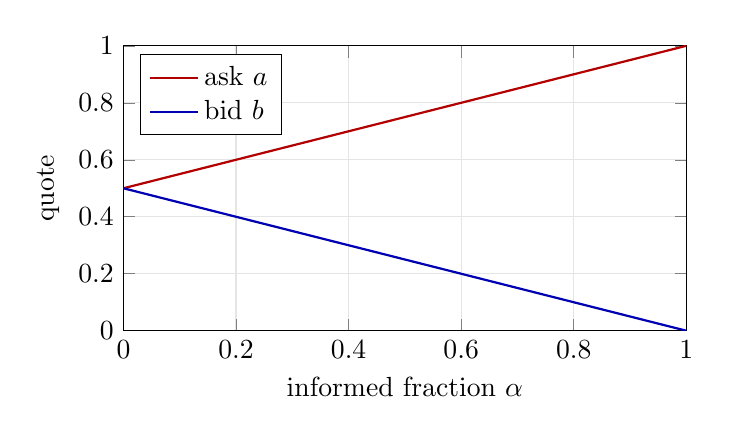
\begin{tikzpicture}
\begin{axis}[width=0.72\linewidth,height=5.2cm,xlabel={informed fraction $\alpha$},ylabel={quote},
  xmin=0,xmax=1,ymin=0,ymax=1,legend pos=north west,legend cell align=left,grid=both,grid style={black!10}]
\addplot[domain=0:1,thick,samples=2,color=red!70!black]{(1+x)/2};
\addplot[domain=0:1,thick,samples=2,color=blue!70!black]{(1-x)/2};
\legend{ask $a$,bid $b$}
\end{axis}
\end{tikzpicture}
\caption{Quotes of the break-even market maker of \cref{ch14:prop-gm}. The gap between the lines is the informed fraction $\alpha$.}
\label{ch14:fig-quotes}
\end{figure}

% ==================================================================
\section{Sizing a bet: the Kelly criterion}\label{ch14:sec-kelly}

A participant who believes $\Prob(A)=p$ while the contract trades at $c<1$ must decide how much to buy. Let wealth be $W$ and
invest a fraction $f\in[0,1)$ of it in Yes contracts at price $c$ (so the number of contracts is $fW/c$). Ignoring fees, wealth after
settlement is
\[
  W\bigl(1+fb\bigr)\ \text{ if }A,\qquad W(1-f)\ \text{ if }A^c,\qquad b=\frac{1-c}{c},
\]
where $b$ is the net odds per unit staked.

\begin{proposition}[Kelly fraction for a binary contract]\label{ch14:prop-kelly}
The expected log growth $g(f)=p\ln(1+fb)+(1-p)\ln(1-f)$ is strictly concave and maximised at
\[
  f^\star=\frac{p-c}{1-c}\qquad(\text{if }p>c;\ f^\star=0\text{ otherwise}).
\]
\end{proposition}
\begin{proof}
$g'(f)=\dfrac{pb}{1+fb}-\dfrac{1-p}{1-f}=0$ gives $pb(1-f)=(1-p)(1+fb)$, i.e.\ $f(pb+(1-p)b)=pb-(1-p)$, so
$f^\star=p-\dfrac{1-p}{b}=p-\dfrac{(1-p)c}{1-c}=\dfrac{p-c}{1-c}$. Concavity: $g''<0$ since both logarithms are concave.
\end{proof}

\begin{example}\label{ch14:ex-kelly}
Let $c=0.55$ and $p=0.65$: $b=0.818$, $f^\star=0.10/0.45=0.222$ and $g(f^\star)=0.0206$ per bet (about $2\%$ of wealth per bet, in
the log sense). Staking half of that, $f=0.111$, still gives $g=0.0153$ (three quarters of the optimal growth) with a much smaller
variance, whereas staking double, $f=0.444$, gives $g=-0.0041<0$: an \emph{over-bet} with a positive edge loses money in the long run.
(Numbers checked numerically.)
\end{example}

\begin{figure}[ht]
\centering
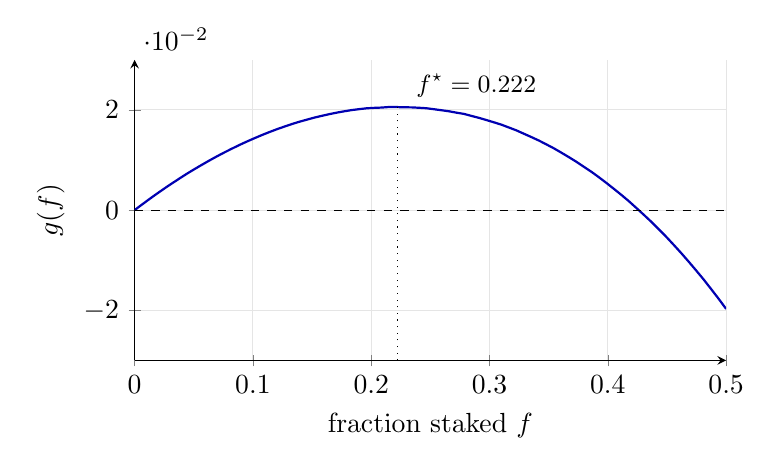
\begin{tikzpicture}
\begin{axis}[width=0.75\linewidth,height=5.4cm,xlabel={fraction staked $f$},ylabel={$g(f)$},
  xmin=0,xmax=0.5,ymin=-0.03,ymax=0.03,grid=both,grid style={black!10},axis lines=left]
\addplot[domain=0:0.5,samples=80,thick,color=blue!70!black]{0.65*ln(1+x*0.81818)+0.35*ln(1-x)};
\draw[dashed] (axis cs:0,0) -- (axis cs:0.5,0);
\draw[dotted] (axis cs:0.2222,-0.03) -- (axis cs:0.2222,0.0206);
\node[anchor=south west,font=\small] at (axis cs:0.23,0.0206) {$f^\star=0.222$};
\end{axis}
\end{tikzpicture}
\caption{Expected log growth for $c=0.55$, $p=0.65$ (\cref{ch14:ex-kelly}). The curve crosses zero at about twice the Kelly fraction.}
\label{ch14:fig-kelly}
\end{figure}

\begin{finance}[Edge and price]
Only the gap $p-c$ matters, scaled by the maximum loss $1-c$: an event contract is the cleanest setting for Kelly, because the outcome
is a genuine Bernoulli variable and the odds are read directly from the price. The estimate of $p$ is itself uncertain, and
$f^\star$ is sensitive to it ($\partial f^\star/\partial p=1/(1-c)$), which is why practitioners use a fraction of Kelly.
\end{finance}

% ==================================================================
\section{Scoring rules, calibration and aggregation}\label{ch14:sec-info}

\paragraph{Brier score.} A forecaster reports $q\in[0,1]$ for an event with outcome $\ind_A$, and is scored by
$(q-\ind_A)^2$ (lower is better). If the true probability is $p$, the expected score is
\[
  \E\,(q-\ind_A)^2 = p(1-q)^2+(1-p)q^2 = p(1-p)+(q-p)^2 .
\]
It is minimised at $q=p$: the Brier score is a \emph{proper} scoring rule, honesty is optimal. For $p=0.6$ the expected scores are
$0.24$ at $q=0.6$, $0.25$ at $q=0.5$ and $0.28$ at $q=0.8$ (verified numerically). The irreducible term $p(1-p)$ is the variance of the event;
only the excess $(q-p)^2$ measures forecasting error. A market price is a forecast, and it is \emph{calibrated} if among all events priced at $q$ a fraction $q$ occur;
comparing a collection of prices with outcomes in this way is how one tests the claim, implicit in the lecture, that an exchange for events makes the
world ``smarter about the future'' \ts{24}{20}{32:38}.

\paragraph{Aggregation of information.} Suppose each of $n$ traders holds an independent private signal $s_i$ about $A$, with likelihood
ratio $\lambda_i=\Prob(s_i\mid A)/\Prob(s_i\mid A^c)$. By Bayes' rule in odds form,
\[
  \frac{\Prob(A\mid s_1,\dots,s_n)}{\Prob(A^c\mid s_1,\dots,s_n)}=\frac{\Prob(A)}{\Prob(A^c)}\prod_i\lambda_i,
\]
so in \emph{log-odds} the evidence adds: $\operatorname{logit}p=\operatorname{logit}p_0+\sum_i\ln\lambda_i$, with $\operatorname{logit}p=\ln\frac p{1-p}$.
With prior $\tfrac12$ and $\lambda=(2,3,1.5)$ the posterior odds are $9$ and $p=0.9$, higher than any single trader would say
(each alone would have $2/3$, $3/4$, $3/5$). The purpose of a market is to make prices carry the pooled log-odds, and
trading is the mechanism: each trader whose belief differs from the price trades, and by \cref{ch14:prop-kelly}
the size of the trade grows with the edge, so the price moves toward the belief-weighted pool. That this works
in practice is an empirical claim, not a theorem: it needs enough liquidity, the market-maker obligations of the previous sections, and traders who cannot manipulate at little cost
(the ``manipulation'' objection heard by the founders \ts{24}{20}{6:22}).

\begin{keyformulas}
\begin{itemize}
  \item Event contract: pays $\ind_A$; price $\pi_A=e^{-rT}\Q(A)\approx\Q(A)$ (\cref{ch14:eq-price}); digital call $D(K)=-\partial C/\partial K$.
  \item No arbitrage: $\sum_\omega\pi_\omega=1$; with a spread, $\sum b_\omega\le1\le\sum a_\omega$ (\cref{ch14:eq-arbband}); thresholds: $P(k)$ non-increasing.
  \item Yes and No: $b^{\mathrm{Yes}}=1-a^{\mathrm{No}}$.
  \item Market maker with informed fraction $\alpha$ (prior $\tfrac12$): $a=\tfrac{1+\alpha}2$, $b=\tfrac{1-\alpha}2$, spread $\alpha$.
  \item Kelly for a contract bought at $c$ with belief $p$: $f^\star=(p-c)/(1-c)$.
  \item Brier: $\E[(q-\ind_A)^2]=p(1-p)+(q-p)^2$.
  \item Independent evidence: $\operatorname{logit}p=\operatorname{logit}p_0+\sum_i\ln\lambda_i$.
  \item From the lecture: cash collateral $100\%$, fee of order $\$1$--$\$2$ per $\$100$, election quotes $\$0.01$ wide with $\$1$M per side.
\end{itemize}
\end{keyformulas}

% ==================================================================
\section*{Exercises}
\addcontentsline{toc}{section}{Exercises}

\begin{exercise}[not from the course]\label{ch14:ex-digital}
In the Black--Scholes model with $r=0$, $C(K)=S\,\Phi(d_1)-K\,\Phi(d_2)$ (\cref{ch:bs}), where $\Phi$ is the standard normal
distribution function. Show that $D(K)=-C'(K)=\Phi(d_2)$, and interpret it as $\Q(S_T>K)$.
\end{exercise}

\begin{exercise}[not from the course]\label{ch14:ex-arb}
Four candidates have asks $0.40,\ 0.30,\ 0.15,\ 0.10$ and bids $0.38,\ 0.28,\ 0.13,\ 0.08$. Is there an arbitrage without fees? With a fee of $1$ cent per
contract bought, how much must the sum of asks fall below $1$ for buying one of each to be profitable?
\end{exercise}

\begin{exercise}[not from the course]\label{ch14:ex-gm}
Generalise \cref{ch14:prop-gm} to a prior $\Prob(V=1)=\pi_0\neq\tfrac12$ and derive the ask and bid. Show that the spread
is $\alpha$ times a factor depending on $\pi_0$, and identify the factor.
\end{exercise}

\begin{exercise}[not from the course]\label{ch14:ex-kellyfee}
A trader believes $p=0.70$ and can buy Yes at $c=0.60$, paying a fee of $0.01$ per contract at purchase. Compute the Kelly fraction with and without the fee (treat the fee as an
increase of the price, $c\to0.61$). By how much does the fee reduce the optimal log growth $g(f^\star)$?
\end{exercise}

\begin{exercise}[not from the course]\label{ch14:ex-portfolio-margin}
Two independent events $A,B$ with $\Prob=\tfrac12$ each. Under full cash collateral, a trader sells Yes on both at price $0.5$. Compute the
locked collateral and the maximum loss of the portfolio. Do the same when $B=A^c$ (compare \cref{ch14:fin-margin}). Explain why the
difference in the required collateral is due to the correlation.
\end{exercise}

\begin{exercise}[not from the course]\label{ch14:ex-brier}
Show that the logarithmic score $-\ln q$ (if $A$) and $-\ln(1-q)$ (if $A^c$) is also proper, and compute its expected value for true probability $p$, in terms of the binary entropy and the Kullback--Leibler divergence.
\end{exercise}
